%!TEX program = xelatex

\documentclass[11pt,titlepage]{report}
%!TEX root = main.tex

\usepackage[T1]{fontenc}
\usepackage{lmodern}
\usepackage[svgnames]{xcolor}
\usepackage{fontspec} % XeLaTeX required!
\usepackage{graphicx}
\usepackage{circuitikz}
\usepackage{tikz}
\usepackage{pifont}
\usepackage[some]{background}
\usepackage{xltxtra} 
\usepackage{setspace}
\usepackage[absolute]{textpos}
\usepackage[latin1]{inputenc}
\usepackage[english]{babel}
\usepackage{graphicx}
\usepackage{wrapfig}
\usepackage{fullpage}
\usepackage[margin=1in]{geometry}
\usepackage{float}
\usepackage{url}
\usepackage{multicol}
\usepackage{hyperref}
\usepackage{titlepic}
\usepackage{standalone}
\usepackage{siunitx}
\usepackage{booktabs}
\usepackage{amsmath}
\usepackage{unicode-math}
\usepackage{verbatim}
\usepackage{enumitem}
\usepackage{listings}
\usepackage{multirow}
\usepackage{pgfplots}
\pgfplotsset{compat=1.8}
\usepackage{caption} 
\usepackage[parfill]{parskip}
\usepackage{import}
\usepackage[backend=bibtexu,texencoding=utf8,bibencoding=utf8,style=ieee,sortlocale=en_GB,language=auto]{biblatex}
\usepackage[strict,autostyle]{csquotes}
\usepackage[final]{pdfpages}
\usepackage{subcaption}
\usepackage{ifplatform}
%\captionsetup[table]{skip=10pt}


% Fix for includepdf bug in Mac OS X
\newcommand{\insertpdfpath}[1]{
	\ifwindows
	\newcommand{\insertpdf}[2]{\includepdf[pages=##1]{##2}}
	\else
	\newcommand{\insertpdf}[2]{\includepdf[pages=##1]{#1/##2}}
	\fi
}

%set fonts
\setmainfont[Ligatures=TeX]{Myriad Pro}
\setmathfont{Asana Math}
\setmonofont{Lucida Console}

\usepackage{titlesec, color}
\renewcommand{\familydefault}{\sfdefault} %set font family
\renewcommand{\arraystretch}{1.2} %set table vertical spacing
\setlength\parindent{0pt} %no paragraph indent
\hypersetup{ %setup hyperlinks
    colorlinks,
    citecolor=black,
    filecolor=black,
    linkcolor=black,
    urlcolor=black
}

%redesign chapter headings
\definecolor{gray75}{gray}{0.75}
\newcommand{\chapternumber}{\thechapter}
\newcommand{\hsp}{\hspace{20pt}}
\titleformat{\chapter}[hang]{\Huge\bfseries}{\chapternumber\hsp\textcolor{gray75}{|}\hsp}{0pt}{\Huge\bfseries}

%Redefine appendix headers
\renewcommand{\appendixname}{Appendix}
\renewcommand{\appendixtocname}{Appendices}
\renewcommand{\appendixpagename}{Appendices}

%For code listings
\definecolor{black}{rgb}{0,0,0}
\definecolor{browntags}{rgb}{0.65,0.1,0.1}
\definecolor{bluestrings}{rgb}{0,0,1}
\definecolor{graycomments}{rgb}{0.4,0.4,0.4}
\definecolor{redkeywords}{rgb}{1,0,0}
\definecolor{bluekeywords}{rgb}{0.13,0.13,0.8}
\definecolor{greencomments}{rgb}{0,0.5,0}
\definecolor{redstrings}{rgb}{0.9,0,0}
\definecolor{purpleidentifiers}{rgb}{0.01,0,0.01}


\lstdefinestyle{csharp}{
language=[Sharp]C,
showspaces=false,
showtabs=false,
breaklines=true,
showstringspaces=false,
breakatwhitespace=true,
escapeinside={(*@}{@*)},
columns=fullflexible,
commentstyle=\color{greencomments},
keywordstyle=\color{bluekeywords}\bfseries,
stringstyle=\color{redstrings},
identifierstyle=\color{purpleidentifiers},
basicstyle=\ttfamily\small}

\lstdefinestyle{c}{
language=C,
showspaces=false,
showtabs=false,
breaklines=true,
showstringspaces=false,
breakatwhitespace=true,
escapeinside={(*@}{@*)},
columns=fullflexible,
commentstyle=\color{greencomments},
keywordstyle=\color{bluekeywords}\bfseries,
stringstyle=\color{redstrings},
identifierstyle=\color{purpleidentifiers},
}

\lstdefinestyle{matlab}{
language=Matlab,
showspaces=false,
showtabs=false,
breaklines=true,
showstringspaces=false,
breakatwhitespace=true,
escapeinside={(*@}{@*)},
columns=fullflexible,
commentstyle=\color{greencomments},
keywordstyle=\color{bluekeywords}\bfseries,
stringstyle=\color{redstrings},
identifierstyle=\color{purpleidentifiers}
}

\lstdefinestyle{vhdl}{
language=VHDL,
showspaces=false,
showtabs=false,
breaklines=true,
showstringspaces=false,
breakatwhitespace=true,
escapeinside={(*@}{@*)},
columns=fullflexible,
commentstyle=\color{greencomments},
keywordstyle=\color{bluekeywords}\bfseries,
stringstyle=\color{redstrings},
identifierstyle=\color{purpleidentifiers}
}

\lstdefinestyle{xaml}{
language=XML,
showspaces=false,
showtabs=false,
breaklines=true,
showstringspaces=false,
breakatwhitespace=true,
escapeinside={(*@}{@*)},
columns=fullflexible,
commentstyle=\color{greencomments},
keywordstyle=\color{redkeywords},
stringstyle=\color{bluestrings},
tagstyle=\color{browntags},
morestring=[b]",
  morecomment=[s]{<?}{?>},
  morekeywords={xmlns,version,typex:AsyncRecords,x:Arguments,x:Boolean,x:Byte,x:Char,x:Class,x:ClassAttributes,x:ClassModifier,x:Code,x:ConnectionId,x:Decimal,x:Double,x:FactoryMethod,x:FieldModifier,x:Int16,x:Int32,x:Int64,x:Key,x:Members,x:Name,x:Object,x:Property,x:Shared,x:Single,x:String,x:Subclass,x:SynchronousMode,x:TimeSpan,x:TypeArguments,x:Uid,x:Uri,x:XData,Grid.Column,Grid.ColumnSpan,Click,ClipToBounds,Content,DropDownOpened,FontSize,Foreground,Header,Height,HorizontalAlignment,HorizontalContentAlignment,IsCancel,IsDefault,IsEnabled,IsSelected,Margin,MinHeight,MinWidth,Padding,SnapsToDevicePixels,Target,TextWrapping,Title,VerticalAlignment,VerticalContentAlignment,Width,WindowStartupLocation,Binding,Mode,OneWay,xmlns:x}
}

\lstdefinestyle{matlab}{
language=Matlab,
showspaces=false,
showtabs=false,
breaklines=true,
showstringspaces=false,
breakatwhitespace=true,
escapeinside={(*@}{@*)},
columns=fullflexible,
commentstyle=\color{greencomments},
keywordstyle=\color{bluekeywords}\bfseries,
stringstyle=\color{purpleidentifiers},
identifierstyle=\color{purpleidentifiers}
}

%defaults
\lstset{
basicstyle=\ttfamily\small,
extendedchars=false,
numbers=left,
numberstyle=\ttfamily\tiny,
stepnumber=1,
tabsize=4,
numbersep=5pt
}
\addbibresource{../../library/bibliography.bib}

\begin{document}

\section{Labday 3}
\subsection{Report 11}
We wanted to investigate the audio channel. For this purpose we used three different signals of which the frequency domain plot is shown in Figure~\ref{fig:rep11-test-spectra}. From the first glance the symilarities between periodic pulses and sines can be seen. Pulses on the frequencies of the signals and mirrored on the negative frequencies. The simmilarities can be explained by the inability of the speakers to give perfect pulses. This was done by sampling higher than the Nyquist frequency though. As expected there is aliasing when sampling under this frequency.  


\begin{figure}[H]
	\centering
	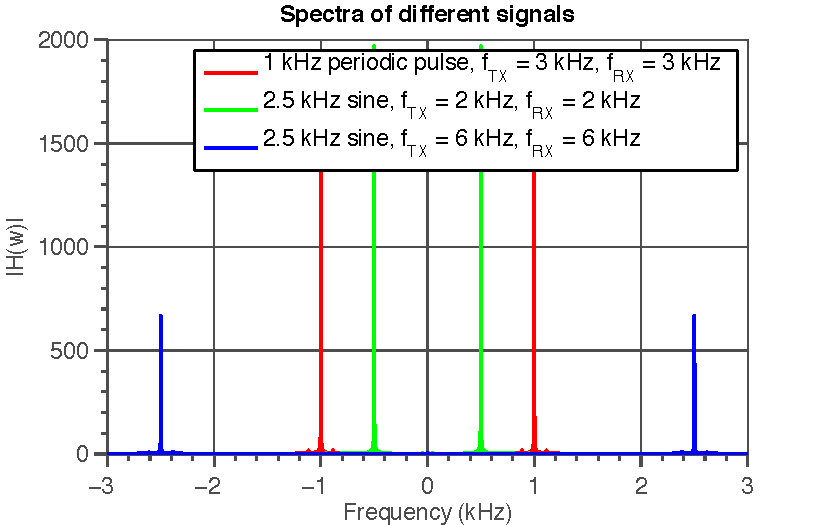
\includegraphics[width=0.6\textwidth]{../../deliverable-7-resources/figures/ass-1/report-11-12-13/ass-1-report-11-random-signals.pdf}
	\caption{Some arbitrary signal spectra, measured in the testing environment}
	\label{fig:rep11-test-spectra}
\end{figure}

The impulse responses and amplitude spectra for which asked in the report are depicted in Figure~\ref{fig:rep11-impulse-spectra}. For $F_s = \SI{22050}{Hz}$ we did not expect any aliasing.  But for $F_{s,TX} = \SI{22050}{Hz}$ and $F_{s,TX} = \SI{8000}{Hz}$ we are sampling under the nyquist frequency, thus some aliasing has to be expected. Finally for $F_{s,TX} = \SI{4000}{Hz}$ and $F_{s,TX} = \SI{22050}{Hz}$ we are sampling above the nyquist frequency. In this case no aliasing is expected and the highest frequency should be $\pm \frac{F_{s,TX}}{2} = \pm \SI{2}{kHz}$. This corresponds considering some noise close enough to our measured spectrum.


\begin{figure}[H]
	\centering
	\begin{subfigure}{0.49\textwidth}
		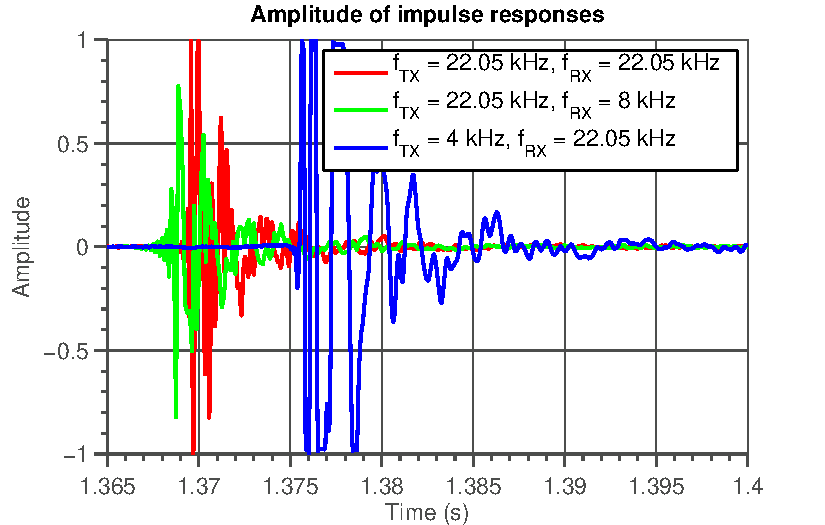
\includegraphics[width=\textwidth]{../../deliverable-7-resources/figures/ass-1/report-11-12-13/ass-1-report-11-time.pdf}
	\end{subfigure}
	\begin{subfigure}{0.49\textwidth}
		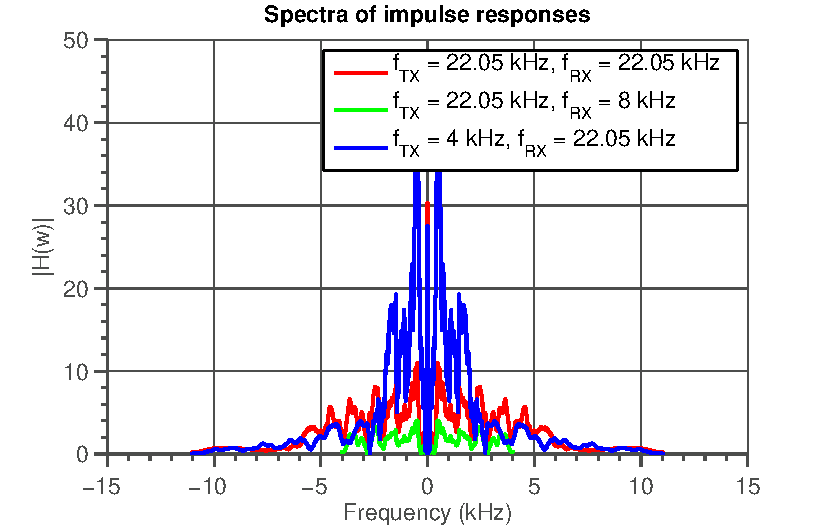
\includegraphics[width=\textwidth]{../../deliverable-7-resources/figures/ass-1/report-11-12-13/ass-1-report-11.pdf}
	\end{subfigure}
	\caption{The required impulse responses and spectra}
	\label{fig:rep11-impulse-spectra}
\end{figure}



\subsection{Report 12}
In order to determine the minimum sample rate which is at least needed to have a resolution of \SI{1}{cm} one have to know the delay. The delay can be calculated with the speed of sound, \SI{340}{m/s}. The delay then becomes $0.01/340 = \SI{29.4}{\micro s}$. From this it follows that $F_s > (29.4 \times 10^{-6})^{-1} = \SI{34}{kHz}$. 

\begin{figure}[H]
	\centering
	\begin{subfigure}{0.49\textwidth}
		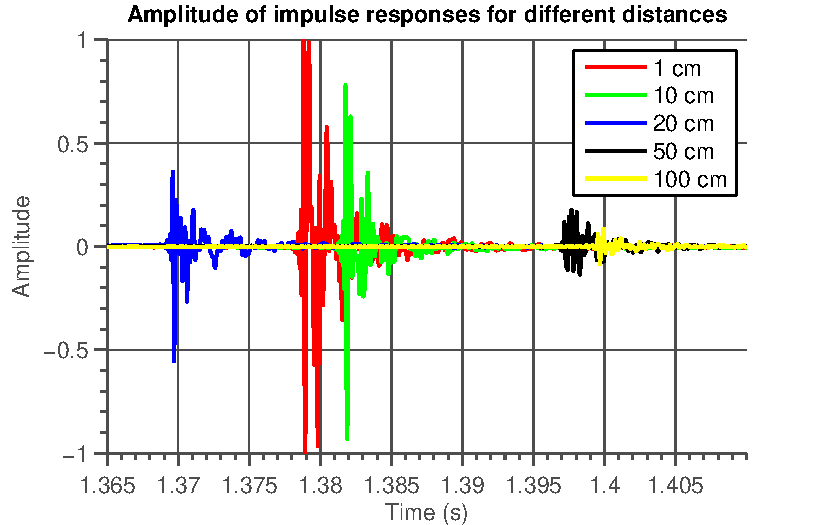
\includegraphics[width=\textwidth]{../../deliverable-7-resources/figures/ass-1/report-11-12-13/ass-1-report-13-time.pdf}
	\end{subfigure}
	\begin{subfigure}{0.49\textwidth}
		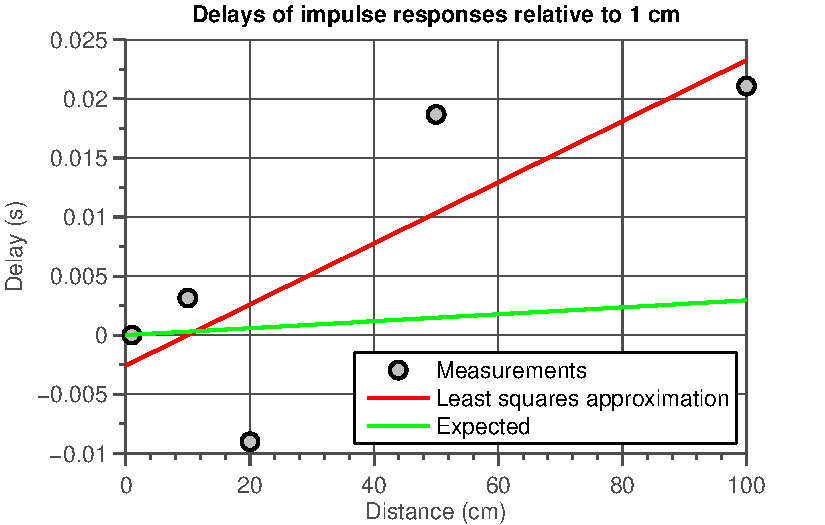
\includegraphics[width=\textwidth]{../../deliverable-7-resources/figures/ass-1/report-11-12-13/ass-1-report-13-delays.pdf}
	\end{subfigure}
	\begin{subfigure}{0.49\textwidth}
		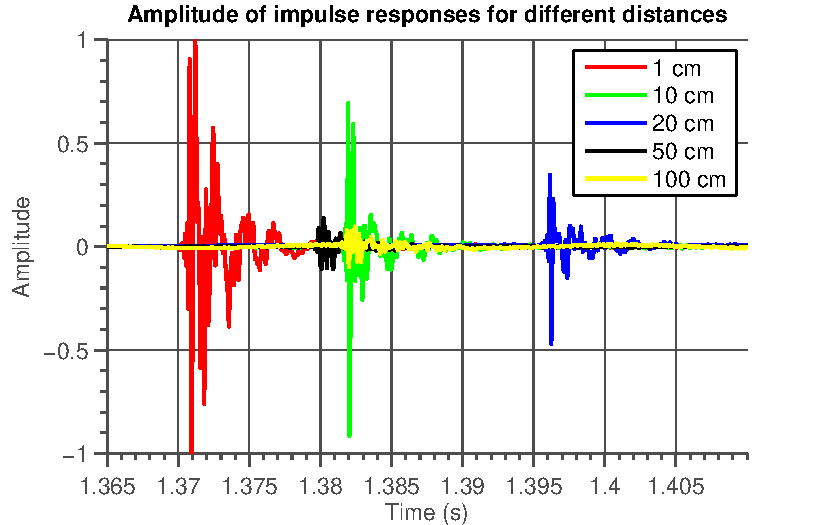
\includegraphics[width=\textwidth]{../../deliverable-7-resources/figures/ass-1/report-11-12-13/ass-1-report-13-time-set-2.pdf}
	\end{subfigure}
	\begin{subfigure}{0.49\textwidth}
		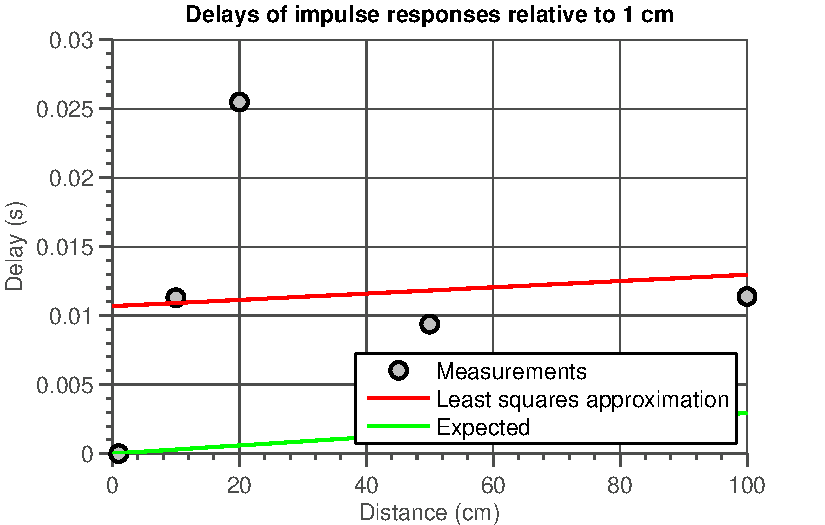
\includegraphics[width=\textwidth]{../../deliverable-7-resources/figures/ass-1/report-11-12-13/ass-1-report-13-delays-set-2.pdf}
	\end{subfigure}
	\caption{Time plots and calculated delays of the received signal, for two different measurements (top and bottom)}
	\label{fig:rep12-los}
\end{figure}

	The received signals after transmitting have been plotted in Figure~\ref{fig:rep12-los}. In this same figure one can see the measured delays with the corresponding distance. Within the latter plot there are also graphs of the least-square approximation and the expecte value. Firstly from the received signals it can be clearly seen that the signals repeat themselves with a demping until becoming zero. Secondly it can be seen form the graphs that the measured delays can differ quit a bit from the expected delay. This is probably a result from signal processing.






\subsection{Report 13}
The measurements of report 12 will now be repeated with an obstacle. The obstacle is a a \SI{15}{"} Macbook. The measurement for \SI{50}{cm} gave logical results. The NLOS signal was delayed and decayed in comparison with the LON signal. For \SI{100}{cm} the results came unexpected. This is because it seems that the NLOS signal arrived earlier, though it was decayed. This unexpected result might be caused once again by processing delays in the receiver. 

\begin{figure}[H]
	\centering
	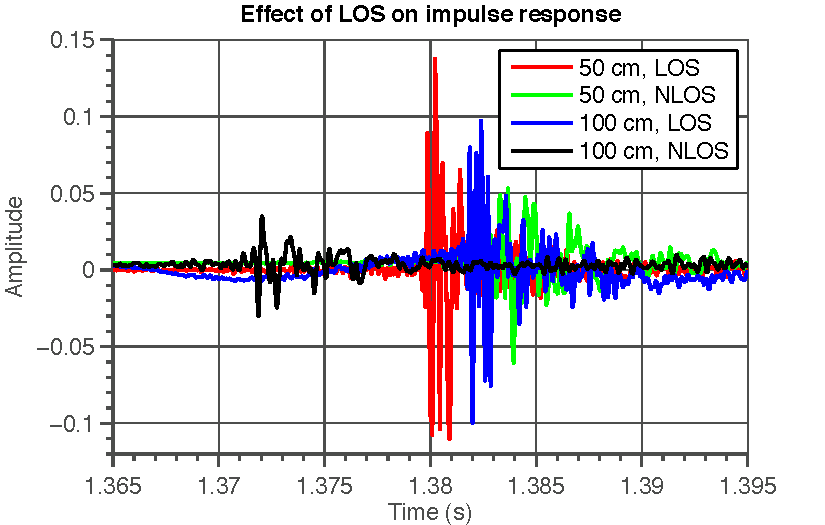
\includegraphics[width=0.8\textwidth]{../../deliverable-7-resources/figures/ass-1/report-11-12-13/ass-1-report-13-los-nlos.pdf}
	\caption{Time plots of received signals with and without line-of-sight}
	\label{fig:rep13-nlos}
\end{figure}





\subsection{Report 14}
In order to test our channel estimation we used \texttt{refsignal.m} to generate signals. The signals where send at different distances, the received signals are shown in Figure~\ref{fig:rep14-tx-rx}. From the received signals we retrieved the impulse responses which are shown in Figure~\ref{fig:rep14-impulse}. With this impulse reponses the signals send where reconstructed. The final results are shown in Figure~\ref{fig:rep14-comparison}. From this plots we can conclude the the our channel estimation works sufficiently well to be used for our TDOA localization. 

\begin{figure}[H]
	\centering
	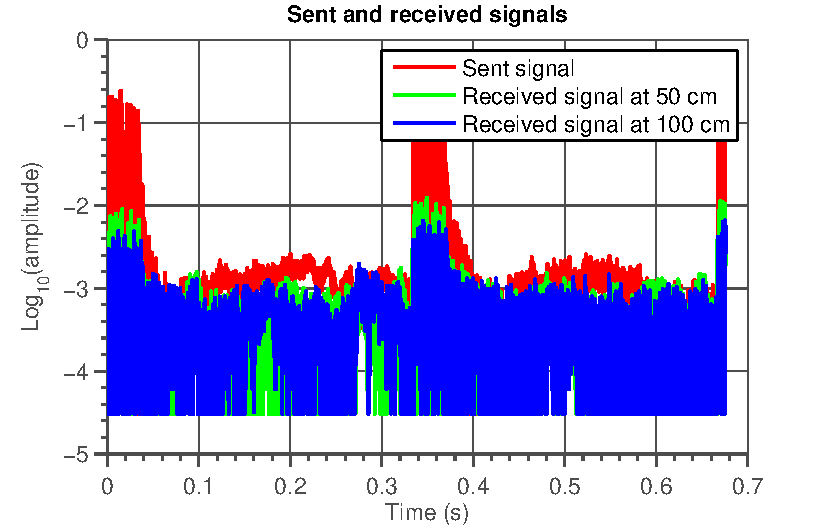
\includegraphics[width=0.8\textwidth]{../../deliverable-7-resources/figures/ass-1/report-14-15/ass-1-report-14-sent-received.pdf}
	\caption{The transmit- and receive sequence}
	\label{fig:rep14-tx-rx}
\end{figure}

\begin{figure}[H]
	\centering
	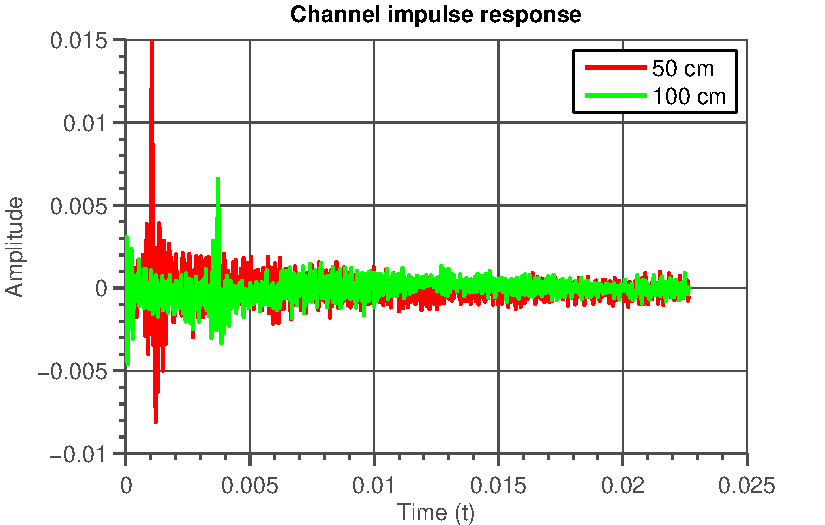
\includegraphics[width=0.8\textwidth]{../../deliverable-7-resources/figures/ass-1/report-14-15/ass-1-report-14-impulse-responses.pdf}
	\caption{The calculated impulse response for measurements, at \SI{50}{cm} and \SI{100}{cm}}
	\label{fig:rep14-impulse}
\end{figure}

\begin{figure}[H]
	\centering
	\begin{subfigure}{0.49\textwidth}
		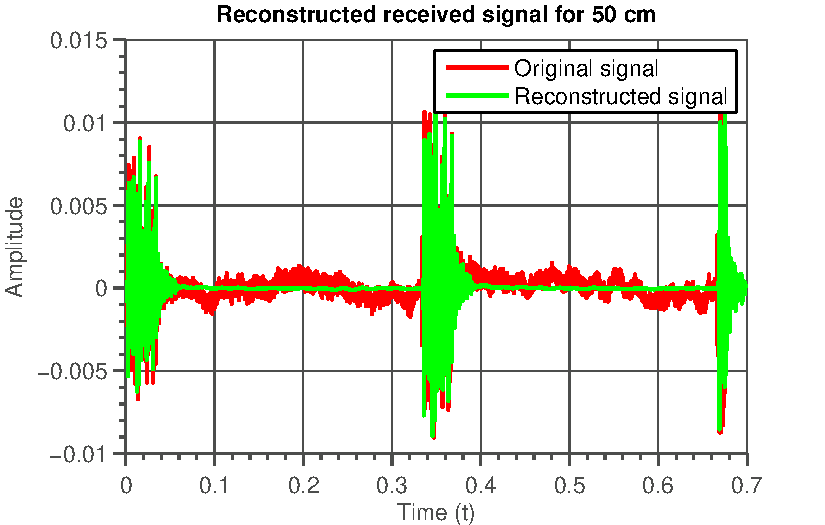
\includegraphics[width=\textwidth]{../../deliverable-7-resources/figures/ass-1/report-14-15/ass-1-report-14-50cm-reconstruction.pdf}
	\end{subfigure}
	\begin{subfigure}{0.49\textwidth}
		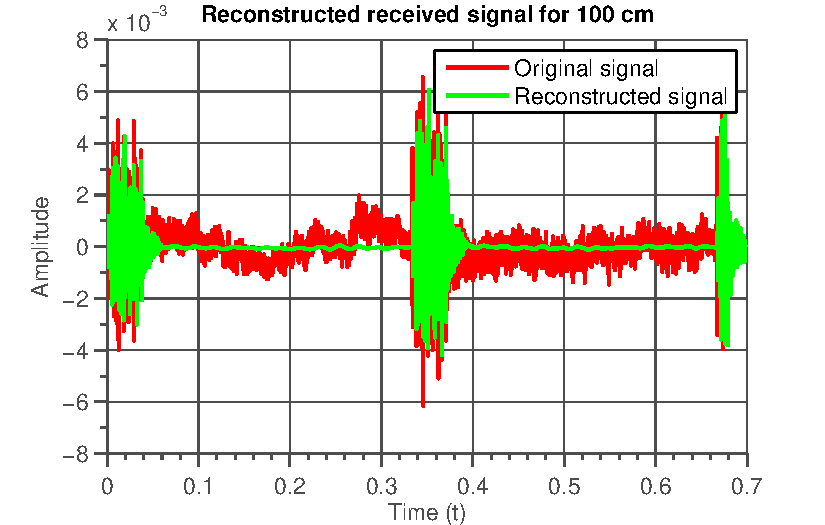
\includegraphics[width=\textwidth]{../../deliverable-7-resources/figures/ass-1/report-14-15/ass-1-report-14-100cm-reconstruction.pdf}
	\end{subfigure}
	\caption{A comparison of the original transmit sequence and the reconstructed transmit sequence, at \SI{50}{cm} and \SI{100}{cm}}
	\label{fig:rep14-comparison}
\end{figure}


\subsection{Report 15}
Design optimal parameters of audio beacon

IK WEET NIET MEER WELKE WAARDES WE HEBBEN GEKOZEN

\end{document}